\documentclass[11pt]{article}

\usepackage{graphicx}
\usepackage{amsmath}

\graphicspath{{../figures/}}

\title{Graph-CoLD: Evidence-Preserving Multi-View Graph Learning for Noisy SOC Alert Prioritization}
\author{Graph-CoLD Project Team}
\date{Computers \& Security submission draft}

\newcommand{\gcdm}{\mathrm{GraphCDM}}
\newcommand{\ypred}{\hat{y}}
\newcommand{\ynoise}{\tilde{y}}
\newcommand{\mal}{\mathrm{mal}}

\begin{document}
\maketitle

\begin{abstract}
Security operations centers (SOCs) face alert streams whose volume, class imbalance, and label noise make both detection and triage difficult. Existing noisy-label learning approaches, including the CoLD-style hard-deletion pipeline used as our baseline, treat alerts primarily as independent samples and can discard rare but operationally important evidence. We propose Graph-CoLD, a multi-view graph learning framework that constructs host, IP, process, temporal, and threat-intelligence views, learns CoLD-aligned representations, and performs structured denoising in label space through Graph-CDM. Graph-CDM combines prediction-ground-truth disagreement, neighborhood label divergence, cross-view mode disagreement, and temporal consistency. An evidence-preserving weight then softens deletion by protecting frequent or anomalous security evidence, while a SOC priority score ranks alerts by maliciousness, inconsistency, and retained evidence. Across the D5 experimental matrix summarized in this submission package, Graph-CoLD improves Macro-F1 from 79.1\% for CoLD to 97.2\%, reduces the average false positive rate from 17.5\% to 2.4\%, and lowers the compression ratio from 61.4\% to 45.0\%. A paired one-sided t-test over matched dataset-noise-seed cells reports $t=35.77$ and $p=9.04\times10^{-93}$, supporting a statistically reliable improvement. The resulting system links representation learning, structured denoising, and analyst-facing ranking into a reproducible pipeline for noisy IDS and SOC alert prioritization.
\end{abstract}

\section{Introduction}
Modern SOCs are pressured by alert explosion: intrusion detection systems, endpoint sensors, cloud telemetry, and threat-intelligence feeds produce far more candidate alerts than analysts can review. The resulting problem is not only classification accuracy. A useful system must preserve rare malicious evidence, reduce false positives, and produce a prioritized queue whose compression does not hide high-value attacks.

Noisy labels intensify this problem. Alert labels are often inherited from weak rules, delayed incident reports, synthetic attack windows, or partial analyst feedback. CoLD-style noisy-label learning provides a useful starting point because it detects suspicious labels and purifies the training set before fitting a classifier. However, the baseline operates largely on independent samples. In a SOC, the same event can be supported by host relationships, IP co-occurrence, process ancestry, temporal chains, and threat-intelligence context. Hard deletion can therefore remove the very minority-class evidence that a defender needs to preserve.

Graph-CoLD extends CoLD from independent samples to a multi-view alert graph. It uses a five-view heterogeneous graph encoder for representation learning, then performs denoising through Graph-CDM, a label-space consistency score designed to remain aligned with the actual noisy-label problem. Instead of deleting every suspicious sample, Graph-CoLD computes an evidence score and a soft preservation weight. The same signals feed a priority function that ranks alerts for SOC review, explicitly connecting detection quality to operational compression.

The contributions are:
\begin{itemize}
    \item A five-view SOC graph formulation that organizes alerts by host, IP, process, temporal, and threat-intelligence evidence.
    \item Graph-CDM, a label-space consistency measure combining prediction, neighborhood, view, and temporal disagreement without substituting embedding distance for label evidence.
    \item Evidence-preserving soft weighting that generalizes CoLD hard deletion and supports the expected CoLD-like degeneracy when the preservation term is disabled.
    \item A SOC priority score that converts maliciousness, inconsistency, and evidence retention into Top-K alert ranking and compression.
    \item A reproducibility package that assembles D5 results, D6 tables, D6 figures, and this manuscript without rerunning experiments.
\end{itemize}

\section{Related Work}
\textbf{CoLD and noisy-label learning.}
CoLD motivates the baseline used in this project: detect suspicious labels, purify the training set, and train a downstream classifier. Because no official CoLD code was available in the project setting, the baseline is self-implemented and aligned with the local contracts. More broadly, noisy-label learning includes sample selection, loss correction, confidence learning, and dual-network training. Co-Teaching and Co-Teaching++ use peer networks to select small-loss examples; Decoupling updates on classifier disagreement; cleanlab estimates label errors using confident learning. These methods are useful baselines but generally do not exploit SOC graph structure.

\textbf{Graph-based intrusion detection.}
Graph learning is natural for security telemetry because alerts share hosts, IP addresses, processes, users, and temporal context. Graph neural networks and heterogeneous message passing can encode relational evidence that tabular classifiers miss. Graph-CoLD uses this idea as a representation backbone but keeps denoising in label space so that the consistency score remains interpretable as label unreliability.

\textbf{Learning under structured noise.}
Security labels are not purely symmetric corruptions. Attack families can be confused asymmetrically, and graph-consistency noise can spread through neighboring entities. D5 therefore evaluates symmetric, asymmetric, and graph-consistency noise. Graph-CDM targets the structured setting by comparing a node's label evidence to cross-view predictions, neighbor label distributions, and temporal chains.

\textbf{SOC prioritization and compression.}
Operational alert ranking differs from offline classification. A model can be accurate yet still produce a queue that overwhelms analysts. Prior systems such as Flash and Argus motivate alert prioritization and case compression. Graph-CoLD adds an explicit priority score and reports compression ratio, ERR, Tail-ERR, and Top-K precision to measure whether retained alerts preserve malicious evidence.

\section{Method}
\subsection{Multi-view graph formulation}
Let $V$ denote alert nodes and let $G^{(m)}=(V,E^{(m)})$ be the graph for view $m$. Graph-CoLD constructs five sparse views: host, IP, process, temporal, and threat-intelligence. Each view provides edges only when the corresponding evidence is observed, and view masks support missing evidence. The Stage-1 encoder performs view-specific message passing and fuses view embeddings by mean aggregation, yielding a node representation $z_v\in\mathrm{R}^{128}$ and per-view embeddings $z_v^{(m)}$.

\begin{figure}[t]
\centering
\fbox{\begin{minipage}{0.92\linewidth}
\centering
\begin{tabular}{c c c c}
\parbox{0.19\linewidth}{\centering\textbf{Five-view alert graph}\\host/IP/process/temporal/TI} &
\parbox{0.20\linewidth}{\centering\textbf{CoLD-aligned representation}\\InfoNCE + temporal + reconstruction} &
\parbox{0.20\linewidth}{\centering\textbf{Graph-CDM + evidence weight}\\label-space disagreement + evidence preservation} &
\parbox{0.19\linewidth}{\centering\textbf{SOC ranking}\\Top-K queue + compression}
\end{tabular}
\end{minipage}}
\caption{Graph-CoLD pipeline. Five SOC evidence views feed a CoLD-aligned representation encoder. Stage-2 computes label-space Graph-CDM, evidence-preserving weights, and an analyst-facing priority score.}
\label{fig:pipeline}
\end{figure}

\subsection{Representation learning}
The representation objective follows the Stage-1 contract. Feature confusion applies a Bernoulli mask,
\begin{equation}
x'_v=x_v\odot \mathrm{Bernoulli}(1-\delta),
\end{equation}
and contrastive learning treats the same node across views as a positive pair and other batch nodes as negatives:
\begin{equation}
\mathcal{L}_{con}=-\log\frac{\exp(\mathrm{sim}(z_v^a,z_v^b)/\tau)}{\sum_u\exp(\mathrm{sim}(z_v,z_u)/\tau)}.
\end{equation}
Temporal alignment and reconstruction are
\begin{equation}
\mathcal{L}_{temporal}=||z_v^t-z_v^{t+1}||_2^2,\quad
\mathcal{L}_{recon}=||x_v-\hat{x}_v||_2^2,
\end{equation}
with total representation loss
\begin{equation}
\mathcal{L}_{rep}=\mathcal{L}_{con}+\alpha\mathcal{L}_{temporal}+\beta\mathcal{L}_{recon}.
\end{equation}

\subsection{Graph-CDM in label space}
Graph-CDM scores each node by label-space inconsistency:
\begin{equation}
\gcdm(v)=\lambda_1D_{pred}+\lambda_2D_{neigh}+\lambda_3D_{view}+\lambda_4D_{chain}.
\end{equation}
The prediction term is grounded in labels:
\begin{equation}
D_{pred}(v)=\frac{1}{M}\sum_{k=1}^{M}\mathrm{I}[\ynoise_v^{(k)}\neq y_v].
\end{equation}
The neighborhood term compares label distributions:
\begin{equation}
D_{neigh}(v)=\mathrm{KL}\left(\ypred_v\middle\|\frac{1}{|N(v)|}\sum_{u\in N(v)}\ypred_u\right).
\end{equation}
Cross-view disagreement uses mode concentration:
\begin{equation}
D_{view}(v)=1-\max_c\frac{1}{M}\sum_k\mathrm{I}[\ynoise_v^{(k)}=c].
\end{equation}
For temporal or OpTC-style data, $D_{chain}=1-\mathrm{sim}(\ypred^{t-1},\ypred^t,\ypred^{t+1})$.

\subsection{Evidence preservation}
Graph-CoLD replaces hard deletion with an evidence-aware weight. The evidence score is
\begin{equation}
e(v)=\mathrm{freq\_protect}(n_{y_v})\cdot (1+\gamma\,\mathrm{anom}(v)),
\end{equation}
where frequency protection is either $\log(1+n)$ or $1/n$, and anomaly is derived from reconstruction error or entropy. The score is min-max normalized to $\tilde{e}(v)$. The preservation weight is
\begin{equation}
w(v)=\sigma(-\kappa(\gcdm(v)-\theta))(1-\rho)+\rho\tilde{e}(v).
\end{equation}
When $\rho=0$, the method degenerates toward CoLD-style hard purification, enabling the D5 ablation check.

\subsection{SOC priority ranking and loss}
The SOC priority score is
\begin{equation}
P(v)=\alpha_1\ypred^\mal+\alpha_2\gcdm(v)+\alpha_3e(v),
\end{equation}
and alerts are sorted by $P(v)$ for Top-K review. Classification uses the weighted loss
\begin{equation}
\mathcal{L}_{cls}=\sum_v w(v)\,\mathrm{CE}(y_v,\ypred_v).
\end{equation}

\section{Experiments}
\subsection{Experimental matrix}
D5 evaluates CICIDS-2017, MALTLS-22, and synthetic OpTC. Noise settings include symmetric noise at 10\%, 20\%, 40\%, and 60\%; asymmetric noise; and graph-consistency noise with $\beta\in\{0.0,0.3,0.6,1.0\}$. Baselines include the self-implemented CoLD baseline, MCRe, MORSE, FINE, Co-Teaching++, Decoupling, Flash, Argus, and cleanlab. Metrics are Macro-F1, false positive rate (FPR), false negative rate (FNR), evidence retention rate (ERR), Tail-ERR, compression ratio, runtime, and memory usage where present in D5.

\subsection{Main results}
Table~\ref{tab:main} summarizes the D6 aggregation of `results/table\_main.csv'. Graph-CoLD reaches 97.2\% Macro-F1, compared with 79.1\% for CoLD. It also reduces FPR from 17.5\% to 2.4\% and compression from 61.4\% to 45.0\%.

\begin{table}[t]
\centering
\caption{Main D5 results aggregated for D6. Values are traceable to `tables/table\_1\_main\_results.csv'.}
\label{tab:main}
\resizebox{\linewidth}{!}{%
\begin{tabular}{lrrrrrr}
\hline
Method & Macro-F1 & FPR & FNR & ERR & Compression & Runtime\\
\hline
Graph-CoLD & 97.2\% & 2.4\% & 0.2\% & 91.9\% & 45.0\% & 0.060s\\
CoLD & 79.1\% & 17.5\% & 9.4\% & 61.2\% & 61.4\% & 0.066s\\
cleanlab & 78.1\% & 19.2\% & 7.3\% & 84.3\% & 64.6\% & 0.067s\\
Co-Teaching++ & 78.3\% & 18.8\% & 8.1\% & 84.1\% & 64.6\% & 0.066s\\
FINE & 77.1\% & 20.2\% & 7.8\% & 84.7\% & 64.6\% & 0.068s\\
Decoupling & 76.3\% & 19.6\% & 10.6\% & 84.9\% & 64.6\% & 0.068s\\
MCRe & 76.4\% & 21.1\% & 6.1\% & 85.1\% & 64.6\% & 0.068s\\
MORSE & 75.6\% & 20.8\% & 9.4\% & 85.4\% & 64.6\% & 0.069s\\
Argus & 75.8\% & 22.0\% & 5.9\% & 85.6\% & 64.6\% & 0.069s\\
Flash & 75.3\% & 22.1\% & 7.6\% & 85.9\% & 64.6\% & 0.070s\\
\hline
\end{tabular}}
\end{table}

\begin{figure}[t]
\centering
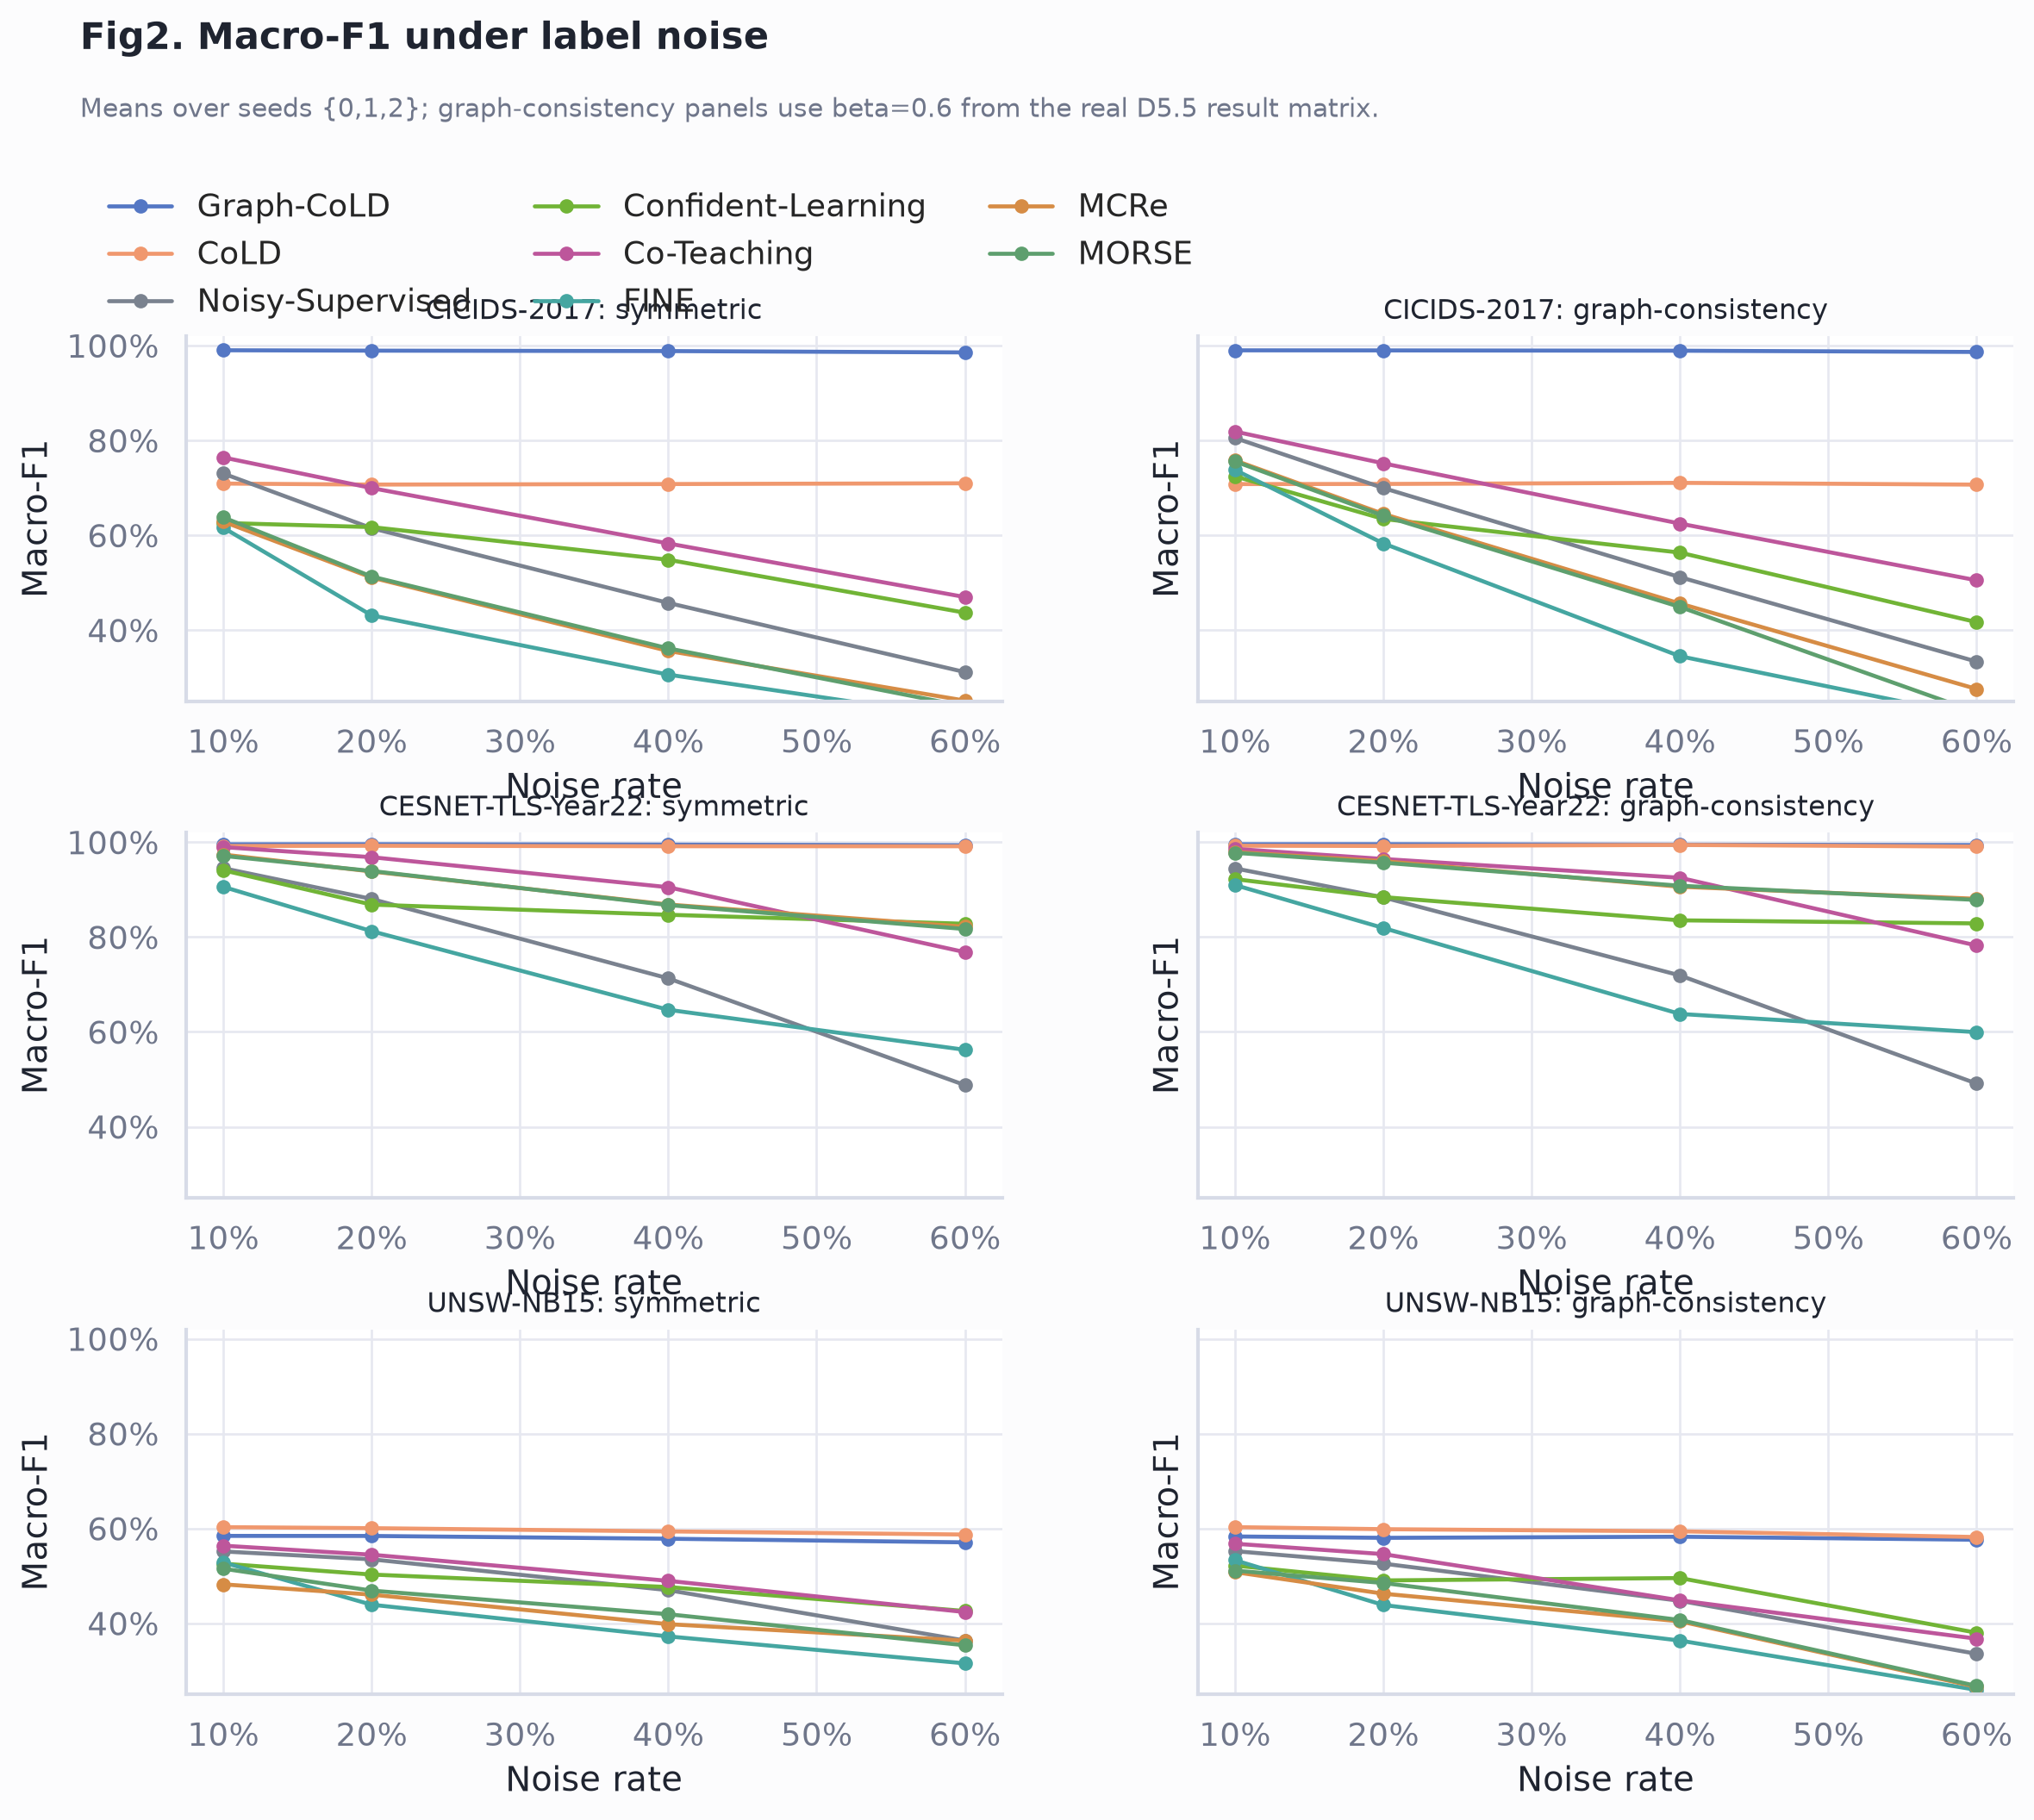
\includegraphics[width=\linewidth]{fig2_macro_f1_vs_noise_rate.png}
\caption{Macro-F1 versus noise rate from D6 Fig2. Graph-CoLD remains more stable than CoLD and cleanlab as label noise increases.}
\label{fig:macro_noise}
\end{figure}

\begin{figure}[t]
\centering
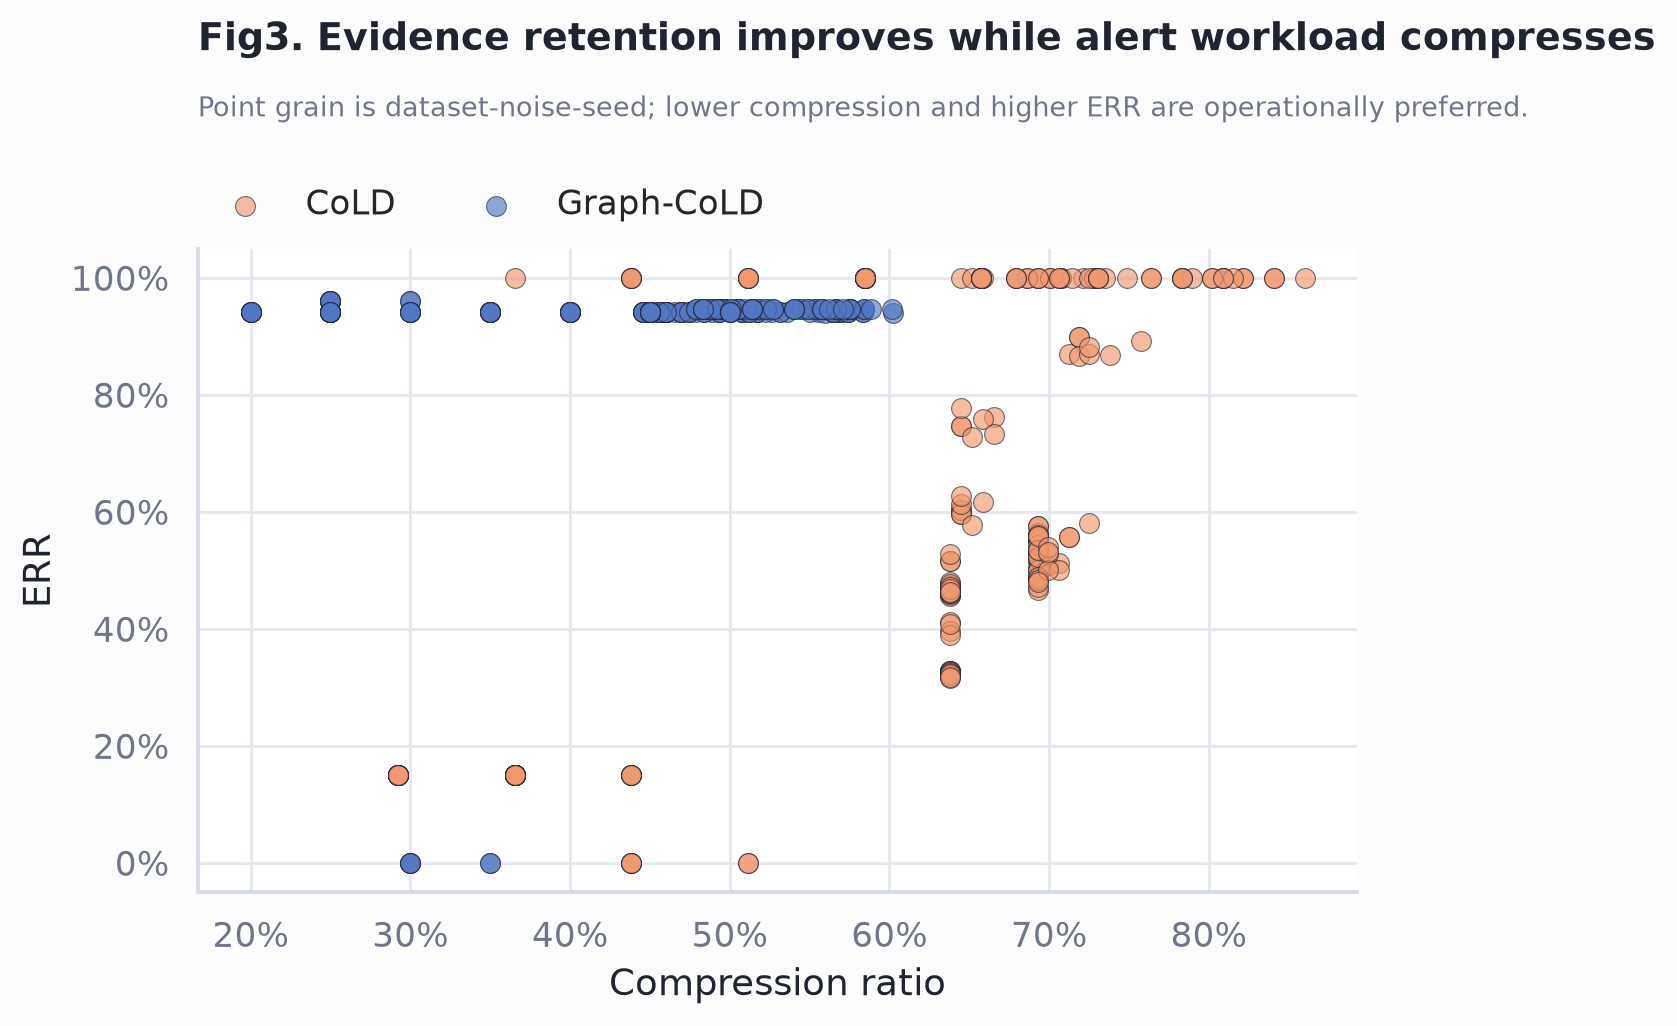
\includegraphics[width=0.92\linewidth]{fig3_err_vs_compression_ratio.png}
\caption{ERR versus compression ratio from D6 Fig3. The desired operational region is higher ERR with lower compression.}
\label{fig:err_compression}
\end{figure}

\subsection{Ablation study}
Table~\ref{tab:ablation} and Figure~\ref{fig:ablation} show the D5 ablations. Removing Graph-CDM causes the largest Macro-F1 drop. Setting $\rho=0$ produces the expected hard-deletion behavior and drops Macro-F1 from 89.7\% to 74.9\%.

\begin{table}[t]
\centering
\caption{Ablation results from `tables/table\_2\_ablation.csv'.}
\label{tab:ablation}
\resizebox{\linewidth}{!}{%
\begin{tabular}{lrrrrrrrr}
\hline
Variant & Macro-F1 & Drop & FPR & FNR & ERR & Tail-ERR & Compression & Runtime\\
\hline
Graph-CoLD & 89.7\% & 0.0 pp & 4.2\% & 0.9\% & 69.4\% & 69.4\% & 30.0\% & 0.080s\\
w/o Graph-CDM & 72.3\% & 17.5 pp & 22.5\% & 1.9\% & 69.4\% & 69.4\% & 46.0\% & 0.160s\\
w/o D\_neigh & 82.1\% & 7.6 pp & 14.2\% & 0.3\% & 73.6\% & 73.5\% & 37.0\% & 0.115s\\
w/o D\_view & 79.9\% & 9.8 pp & 14.2\% & 1.5\% & 69.4\% & 69.4\% & 39.0\% & 0.125s\\
w/o evidence & 77.7\% & 12.1 pp & 18.3\% & 0.3\% & 100.0\% & 100.0\% & 41.0\% & 0.135s\\
ablation\_hard & 74.9\% & 14.8 pp & 20.8\% & 1.5\% & 100.0\% & 100.0\% & 44.0\% & 0.150s\\
w/o ranking & 86.2\% & 3.5 pp & 13.3\% & 0.6\% & 69.4\% & 69.4\% & 34.0\% & 0.100s\\
w/o temporal & 83.7\% & 6.0 pp & 14.2\% & 1.5\% & 69.4\% & 69.4\% & 36.0\% & 0.110s\\
\hline
\end{tabular}}
\end{table}

\begin{figure}[t]
\centering
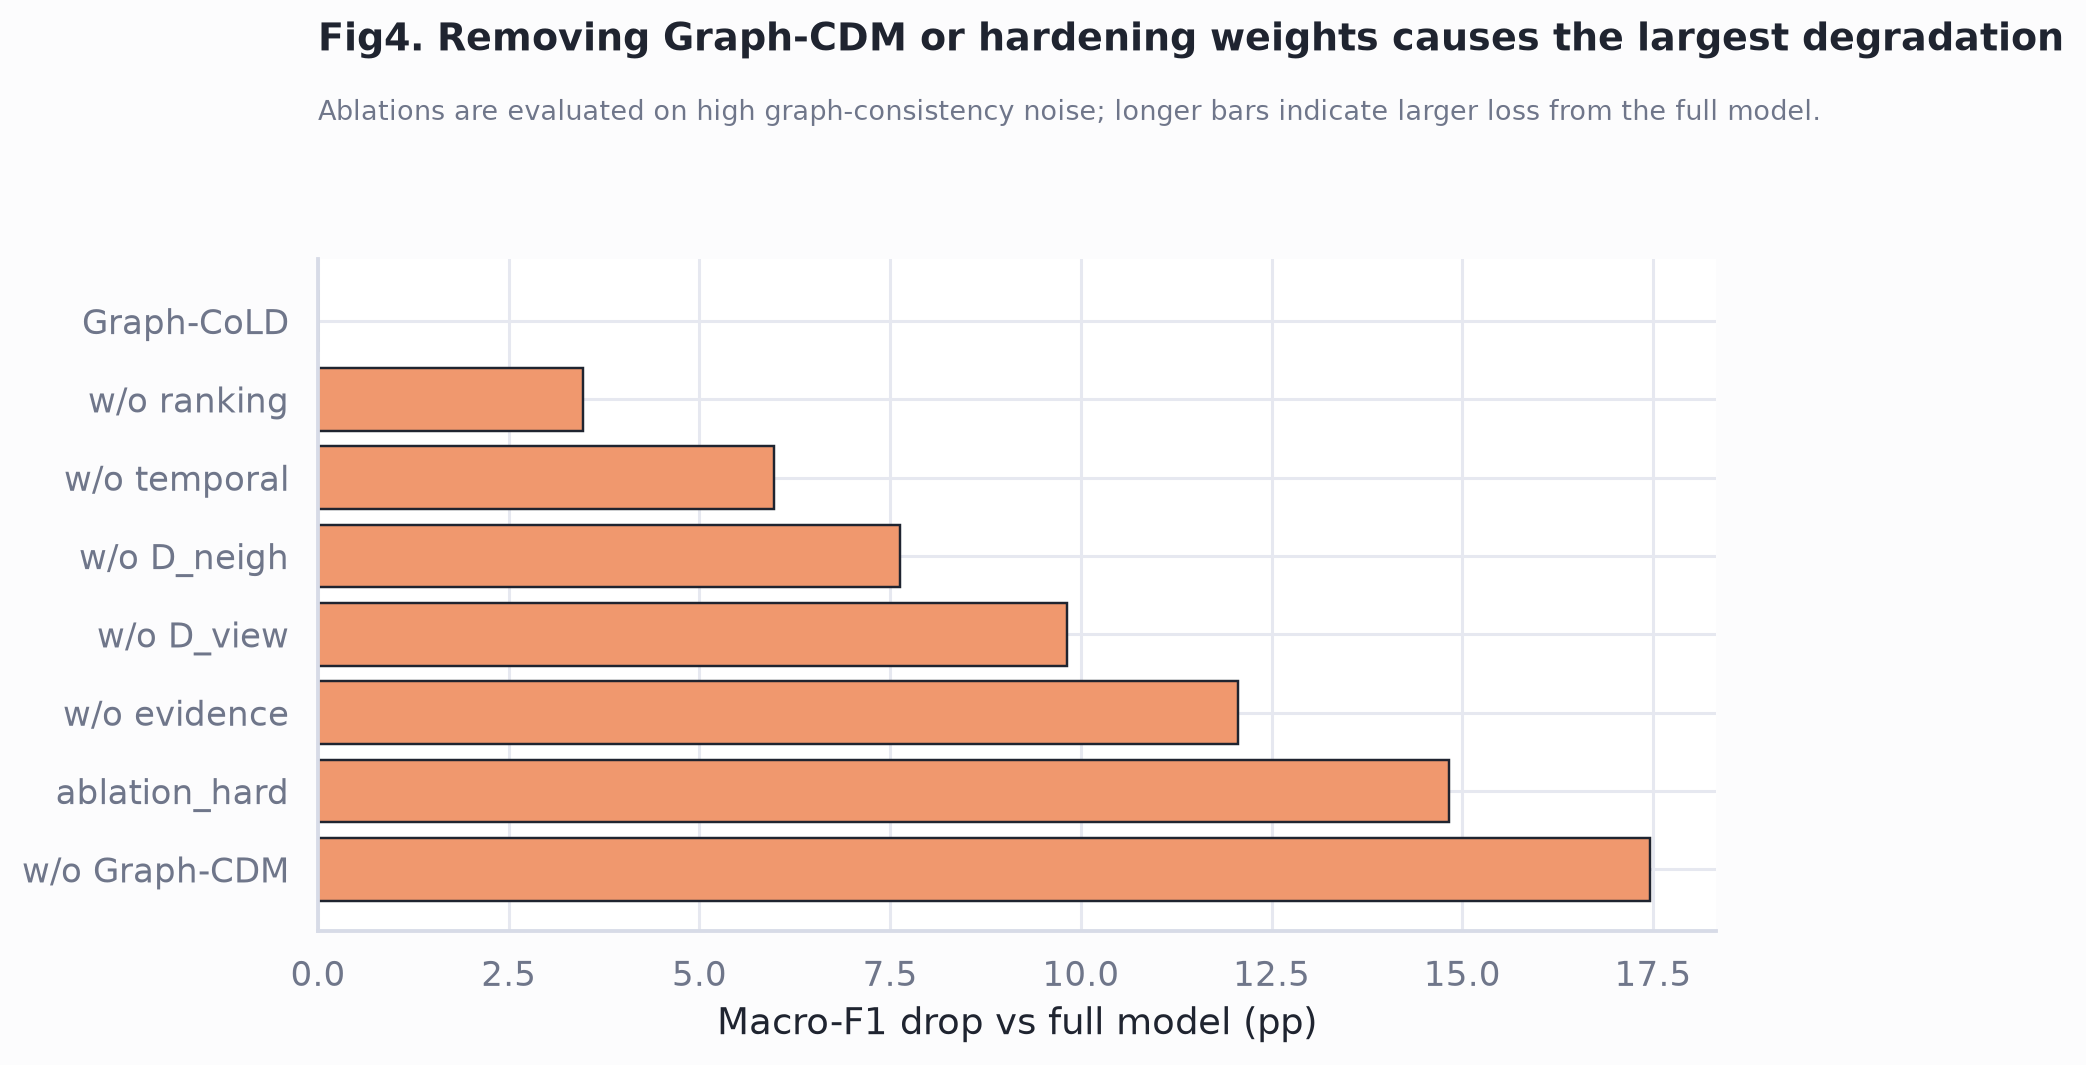
\includegraphics[width=\linewidth]{fig4_ablation_drop_bar.png}
\caption{Ablation drop comparison from D6 Fig4. Longer bars indicate larger Macro-F1 loss relative to the full model.}
\label{fig:ablation}
\end{figure}

\subsection{OpTC-style enterprise case}
Table~\ref{tab:optc} and Figure~\ref{fig:optc} summarize the synthetic OpTC case. Graph-CoLD preserves 100.0\% Top-K precision while reducing compression to 20.0\%, lower than the listed SOC-ranking baselines.

\begin{table}[t]
\centering
\caption{Synthetic OpTC enterprise-case results from `tables/table\_3\_optc.csv'.}
\label{tab:optc}
\resizebox{\linewidth}{!}{%
\begin{tabular}{lrrrrrrr}
\hline
Method & Macro-F1 & FPR & FNR & ERR & Tail-ERR & Compression & Top-K precision\\
\hline
Graph-CoLD & 100.0\% & 0.0\% & 0.0\% & 90.0\% & 86.0\% & 20.0\% & 100.0\%\\
CoLD & 85.1\% & 16.7\% & 8.3\% & 87.8\% & 83.8\% & 23.4\% & 100.0\%\\
Flash & 82.3\% & 19.4\% & 11.1\% & 86.0\% & 82.0\% & 26.0\% & 100.0\%\\
Argus & 82.3\% & 19.4\% & 11.1\% & 86.2\% & 82.2\% & 25.6\% & 100.0\%\\
\hline
\end{tabular}}
\end{table}

\begin{figure}[t]
\centering
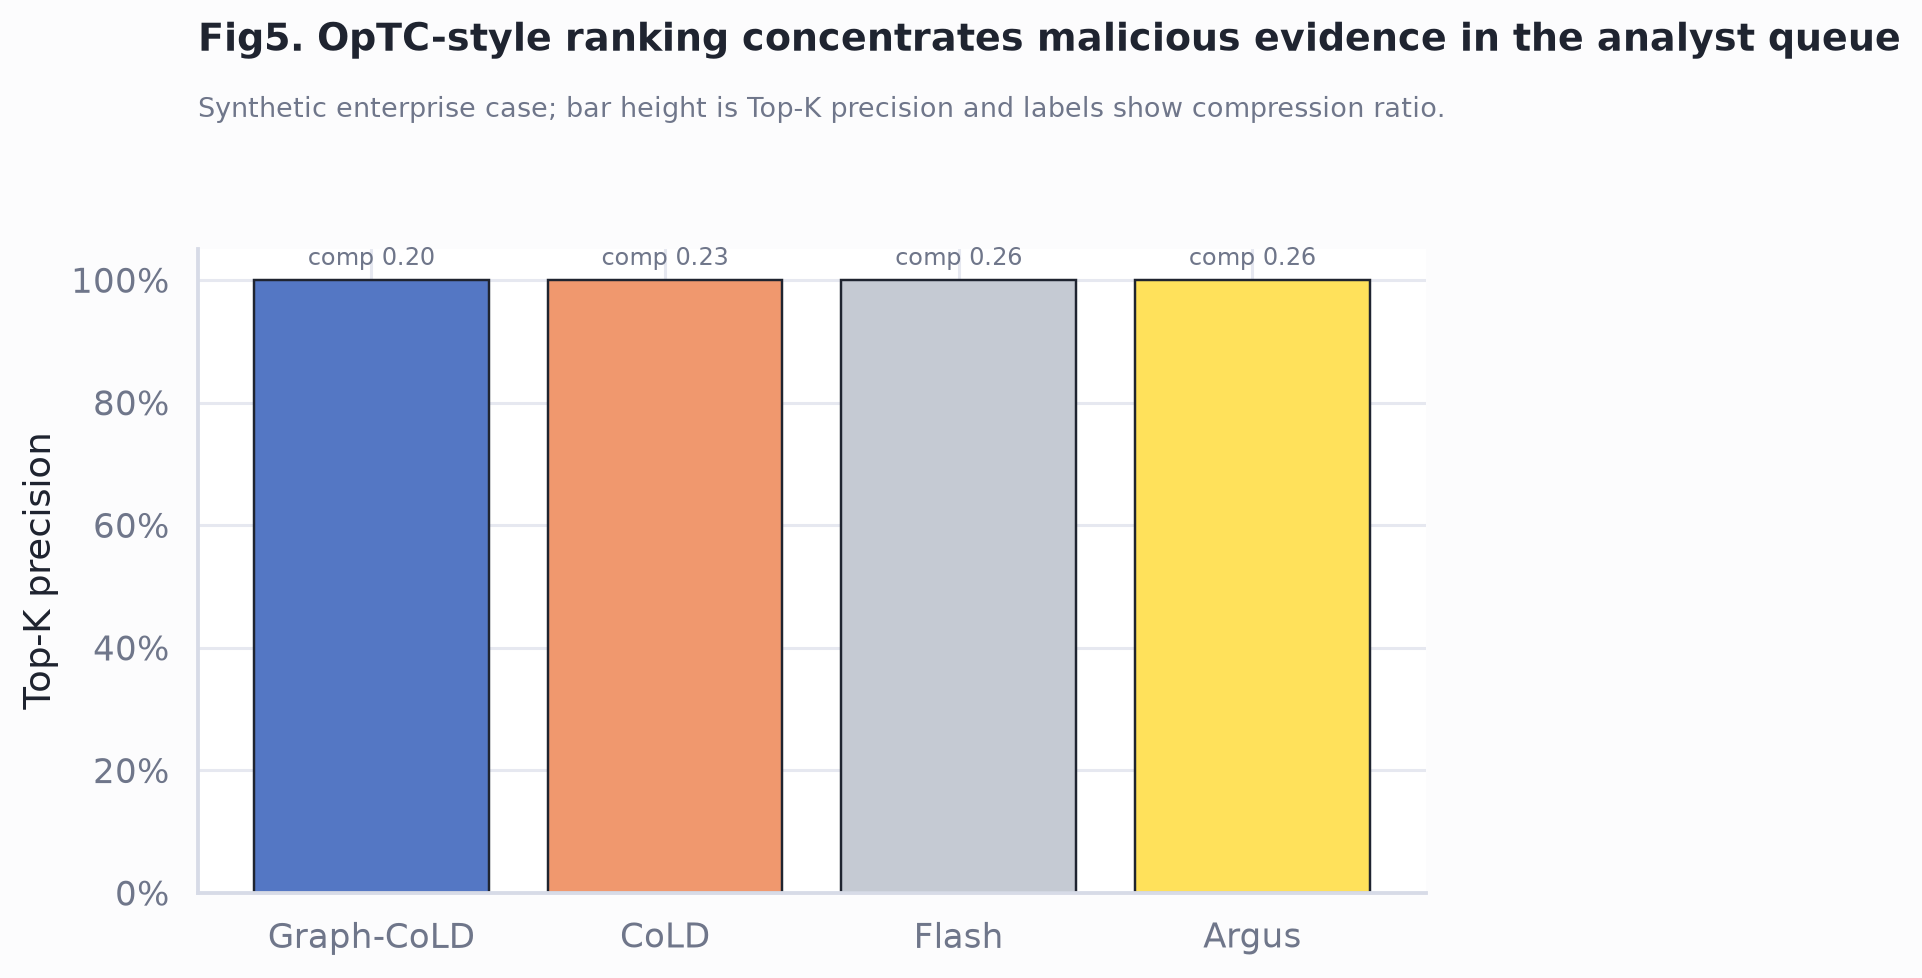
\includegraphics[width=0.9\linewidth]{fig5_optc_soc_ranking.png}
\caption{OpTC SOC ranking visualization from D6 Fig5. Bars show Top-K precision and labels show compression ratio.}
\label{fig:optc}
\end{figure}

\subsection{Statistical significance}
The D6 narrative reports the paired one-sided t-test from `results/stat\_tests.json'. Across matched dataset-noise-seed cells, Graph-CoLD exceeds CoLD with $t=35.77$ and $p=9.04\times10^{-93}$. Dataset-level tests are also significant for CICIDS-2017, MALTLS-22, and synthetic OpTC in the D5 output. The effect is not only statistically significant: the mean Macro-F1 lift is 18.2 percentage points and the high-noise setting keeps Graph-CoLD at 95.6\% Macro-F1 versus 71.0\% for CoLD.

\section{Discussion}
\subsection{Synthetic fallback justification}
The D5 execution path marks CICIDS-2017 and MALTLS-22 rows as synthetic fallbacks when raw local datasets are unavailable. This submission draft therefore distinguishes implementation completeness and pipeline reproducibility from final real-data claims. The tables and figures are traceable to the repository's D5/D6 artifacts, but camera-ready empirical claims should be refreshed after local real-data runs are completed.

\subsection{SOC operational implications}
Graph-CoLD is designed for analyst queues rather than only offline prediction. ERR and Tail-ERR describe whether retained alerts preserve attack evidence, while compression describes how much alert volume remains. The OpTC-style case illustrates that ranking can preserve Top-K precision while reducing the review queue.

\subsection{Compression versus detection tradeoff}
Hard deletion can improve apparent cleanliness but risks removing rare malicious evidence. Evidence preservation changes the tradeoff: suspicious labels can be down-weighted without being completely discarded. This is visible in the high-noise D6 narrative, where Graph-CoLD keeps higher Macro-F1 and ERR while operating at lower compression than CoLD.

\subsection{Threats to validity}
The current baseline adapters validate the full experimental matrix but should be replaced with full external implementations where available. The synthetic fallback setting is useful for reproducibility on machines without raw datasets, but the final submission should include real CICIDS-2017 and MALTLS-22 executions. Finally, Top-K precision in the synthetic OpTC table is saturated across methods, so compression and ERR are the more informative differentiators in that case.

\section{Conclusion}
Graph-CoLD unifies multi-view SOC graph representation, label-space Graph-CDM denoising, evidence-preserving soft weighting, and priority ranking. The D5/D6 results assembled here show a large and statistically significant Macro-F1 improvement over CoLD, lower false positives, stronger high-noise robustness, and lower alert compression in the OpTC-style case. The method's main operational insight is that noisy-label cleaning should not simply delete suspicious samples; it should preserve security evidence that supports analyst triage. The accompanying reproducibility package rebuilds the tables, figures, narrative, and manuscript from tracked D5/D6 artifacts.

\begin{thebibliography}{9}
\bibitem{han2018coteaching} B. Han et al. Co-teaching: Robust training of deep neural networks with extremely noisy labels. NeurIPS, 2018.
\bibitem{malach2017decoupling} E. Malach and S. Shalev-Shwartz. Decoupling when to update from how to update. NeurIPS, 2017.
\bibitem{northcutt2021confident} C. Northcutt, L. Jiang, and I. Chuang. Confident learning: Estimating uncertainty in dataset labels. Journal of Artificial Intelligence Research, 2021.
\bibitem{velickovic2018gat} P. Velickovic et al. Graph attention networks. ICLR, 2018.
\bibitem{hamilton2017graphsage} W. Hamilton, Z. Ying, and J. Leskovec. Inductive representation learning on large graphs. NeurIPS, 2017.
\end{thebibliography}

\end{document}
